Le porte logiche sono particolari meccanismi che applicano trasformazioni a bit o qubit (o coppie di essi) e sono quindi la base di tutte le operazioni complesse svolte dalle macchine di Turing, classiche o quantistiche che siano.
\section{Classiche (1 bit)}
\subsection{NOT}
\begin{center}
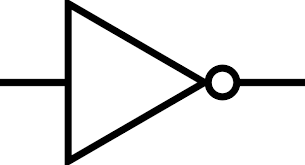
\includegraphics[scale=0.7]{notGate}
\end{center}
La porta logica \textit{NOT} ha in ingresso un segnale e manda in uscita il suo opposto.\\
Mappa quindi:
$0\rightarrow1$ e $1\rightarrow0$.
\section{Classiche (2 bit)}
\subsection{AND}
\begin{center}
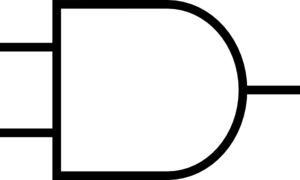
\includegraphics[scale=12]{andGate}
\end{center}
La porta logica \textit{AND} ha in ingresso due segnali e manda in uscita un segnale positivo se e solo se entrambi sono positivi.\\
Mappa quindi:\\
$\{1,1\}\rightarrow1$, $\{1,0\}\rightarrow0$, $\{0,1\}\rightarrow0,$ $\{0,0\}\rightarrow0$
\subsection{OR}
\begin{center}
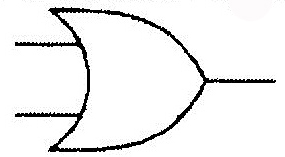
\includegraphics[scale=3]{orGate}
\end{center}
La porta logica \textit{OR} ha in ingresso due segnali e manda in uscita un segnale positivo se almeno uno è positivo.\\
Mappa quindi:\\
$\{1,1\}\rightarrow1$, $\{1,0\}\rightarrow1$, $\{0,1\}\rightarrow1,$ $\{0,0\}\rightarrow0$
\subsection{XOR}
\begin{center}
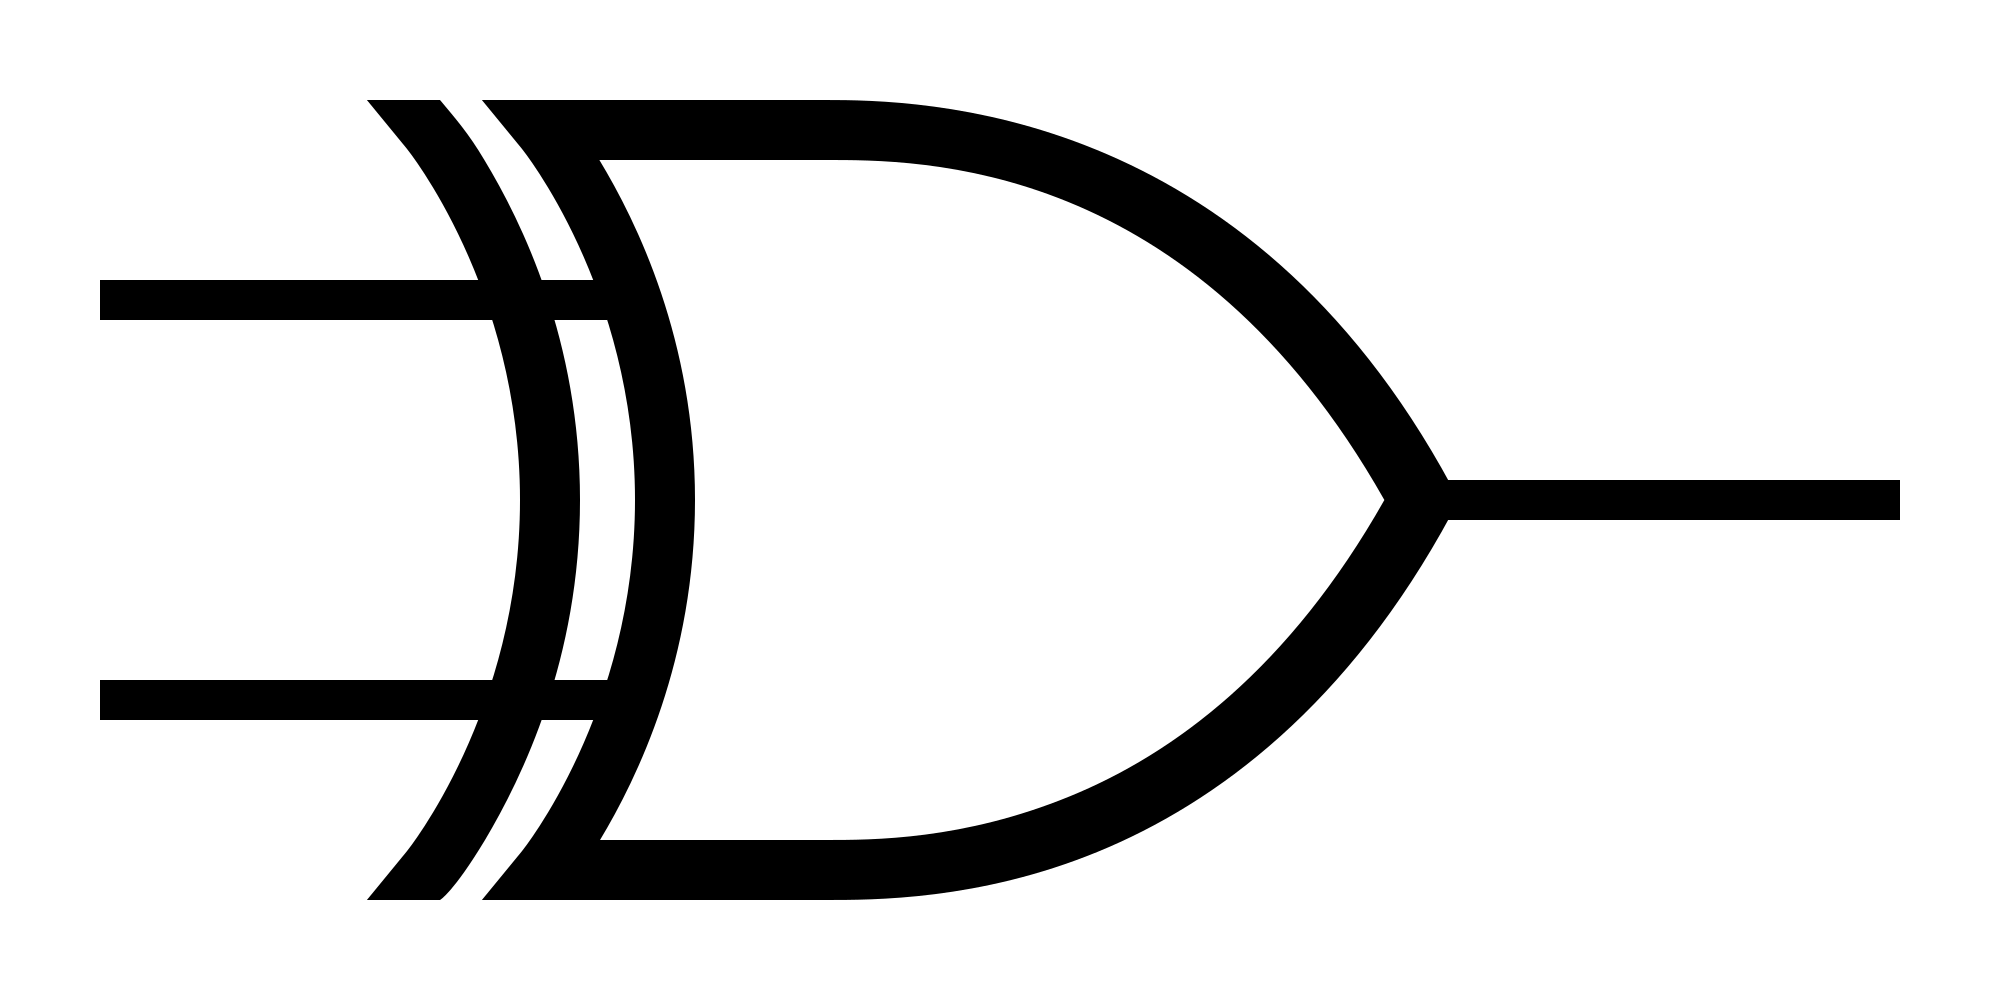
\includegraphics[scale=0.15]{xorGate}
\end{center}
La porta logica \textit{XOR} ha in ingresso due segnali e manda in uscita un segnale positivo se e solo se solo uno è positivo.\\
Mappa quindi:\\
$\{1,1\}\rightarrow0$, $\{1,0\}\rightarrow1$, $\{0,1\}\rightarrow1,$ $\{0,0\}\rightarrow0$
\subsection{Altre}
Esistono poi altre porte logiche, come la NAND o la NOR; ma non sono fondamentali in quanto ottenibili da una combinazione di quelle mostrate (ad esempio NAND = AND + NOT).\\
Porte logiche con più di due segnali di ingresso non vengono usate in quanto per computare più informazioni è sufficiente concatenare.
\section{Quantistiche (1 qubit)}
\subsection{Measurment}
\subsection{X}
\subsection{Hadamard}
\subsection{Z}
\subsection{S}
\subsection{T}
\section{Quantistiche (2 qubit)}
\subsection{CNOT}